\documentclass{article}
\usepackage[mast]{lucky}

\title{Constructing Auxillary Figures}
\author{Dennis Chen}
\date{GPU}

\begin{document}
\maketitle

The whole premise of this handout is that you just construct something else, and the problem instantly becomes clear.

\pagebreak

\section{Problems}

\psetquote{Memories aren't something you can go out of your way to create. It's what's left over!}{Yugami-kun}

\begin{prob}[AIME II 2007/3]{2}
Square $ABCD$ has side length $13$, and points $E$ and $F$ are exterior to the square such that $BE=DF=5$ and $AE=CF=12$. Find $EF^{2}$.
\end{prob}

\begin{req}[]{2}
Let $ABCD$ be a square and $P$ be a point outside of $ABCD$ such that $\angle APB=90^{\circ}.$ Prove that the bisector of $\angle APB$ bisects $ABCD$ into two polygons of equal area.
\end{req}

\begin{prob}[PUMaC 2015]{2}
Find the distance $\overline{CF}$ in the diagram below where $ABDE$ is a square and angles and lengths are as given:
\begin{center}
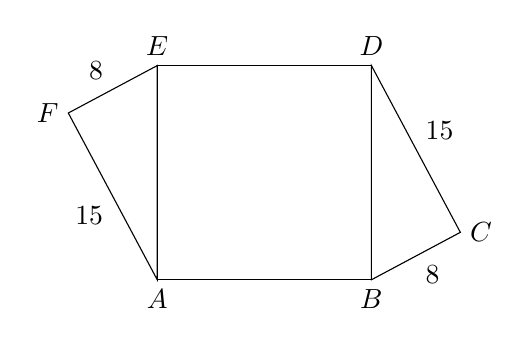
\begin{tikzpicture}[scale=0.16]
\draw (0,0)--(17,0)--(17,17)--(0,17)--cycle;
\draw (0,17)--(-120/17,225/17)--(0,0)--cycle;
\draw (17,17)--(17+120/17,64/17)--(17,0)--cycle;
\node at (0,0) [anchor=north]{$A$};
\node at (17,0) [anchor=north]{$B$};
\node at (17+120/17,64/17) [anchor=west]{$C$};
\node at (17,17) [anchor=south]{$D$};
\node at (0,17) [anchor=south]{$E$};
\node at (-120/17,225/17) [anchor=east]{$F$};
\node at (-60/17,17/2+225/34) [anchor=south east]{$8$};
\node at (-60/17,225/34) [anchor=north east]{$15$};
\node at (17+60/17,32/17) [anchor=north west]{$8$};
\node at (17+60/17,17/2+32/17) [anchor=south west]{$15$};

\coordinate (A) at (0,0) {};
\coordinate (F) at (-120/17,225/17) {};
\coordinate (E) at (0,17) {};

\coordinate (B) at (17,0) {};
\coordinate (C) at (17+120/17,64/17) {};
\coordinate (D) at (17,17) {};

\tkzMarkRightAngle[size=1.5](A,F,E);
\tkzMarkRightAngle[size=1.5](D,C,B);
\end{tikzpicture}
\end{center}
The length $\overline{CF}$ is of the form $a\sqrt{b}$ for integers $a, b$ such that no integer square greater than $1$ divides $b$. What is $a + b$?
\end{prob}

\begin{prob}[AMC 8 2017/25]{3}
One-inch squares are cut from the corners of this 5 inch square.  What is the area in square inches of the largest square that can be fitted into the remaining space?

\begin{center}
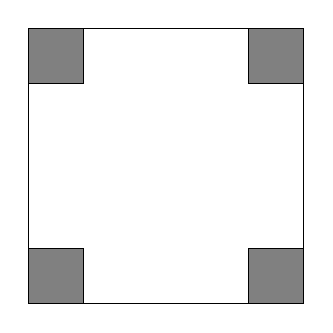
\begin{tikzpicture}[scale=0.7]
\filldraw[gray] (0,4)--(1,4)--(1,5)--(0,5)--cycle;
\filldraw[gray] (0,0)--(1,0)--(1,1)--(0,1)--cycle;
\filldraw[gray] (4,0)--(4,1)--(5,1)--(5,0)--cycle;
\filldraw[gray] (4,4)--(4,5)--(5,5)--(5,4)--cycle;
\draw (0,4)--(1,4)--(1,5)--(0,5)--cycle;
\draw (0,0)--(1,0)--(1,1)--(0,1)--cycle;
\draw (4,0)--(4,1)--(5,1)--(5,0)--cycle;
\draw (4,4)--(4,5)--(5,5)--(5,4)--cycle;
\draw (0,0)--(0,5)--(5,5)--(5,0)--cycle;
\end{tikzpicture}
\end{center}

\end{prob}

\begin{prob}[AIME II 2008/5]{3}
In trapezoid $ABCD$ with $\overline{BC}\parallel\overline{AD}$, let $BC = 1000$ and $AD = 2008$. Let $\angle A = 37^\circ$, $\angle D = 53^\circ$, and $M$ and $N$ be the midpoints of $\overline{BC}$ and $\overline{AD}$, respectively. Find the length $MN$.
\end{prob}

\begin{prob}[Kyiv City Math Olympiad 2014/7.4]{4}
Consider simple convex quadrilateral $ABCD$ where $AD=AB+CD.$ If the angle bisectors of $\angle BAD$ and $\angle CAD$ intersect at $P$, prove that $BP=CP.$ % https://artofproblemsolving.com/community/c4h2223166_bpcp_when_adabcd_angle_bisectors_related_in_abcd_2014_kyiv_city_mo_74
\end{prob}

\begin{req}[AMC 10B 2020/21]{9}
In square $ABCD$, points $E$ and $H$ lie on $\overline{AB}$ and $\overline{DA}$, respectively, so that $AE=AH.$ Points $F$ and $G$ lie on $\overline{BC}$ and $\overline{CD}$, respectively, and points $I$ and $J$ lie on $\overline{EH}$ so that $\overline{FI} \perp \overline{EH}$ and $\overline{GJ} \perp \overline{EH}$. See the figure below. Triangle $AEH$, quadrilateral $BFIE$, quadrilateral $DHJG$, and pentagon $FCGJI$ each has area $1.$ What is $FI^2$?
\end{req}

\begin{center}
\begin{asy}
real x=2sqrt(2); real y=2sqrt(16-8sqrt(2))-4+2sqrt(2); real z=2sqrt(8-4sqrt(2)); pair A, B, C, D, E, F, G, H, I, J; A = (0,0); B = (4,0); C = (4,4); D = (0,4); E = (x,0); F = (4,y); G = (y,4); H = (0,x); I = F + z * dir(225); J = G + z * dir(225); draw(A--B--C--D--A); draw(H--E); draw(J--G^^F--I); draw(rightanglemark(G, J, I), linewidth(.5)); draw(rightanglemark(F, I, E), linewidth(.5)); dot("$A$", A, S); dot("$B$", B, S); dot("$C$", C, dir(90)); dot("$D$", D, dir(90)); dot("$E$", E, S); dot("$F$", F, dir(0)); dot("$G$", G, N); dot("$H$", H, W); dot("$I$", I, SW); dot("$J$", J, SW);
\end{asy}
\end{center}

\begin{prob}[ISL 2001/G1]{13}
Let $A_1$ be the center of the square inscribed in acute triangle $ABC$ with two vertices of the square on side $BC$. Thus one of the two remaining vertices of the square is on side $AB$ and the other is on $AC$. Points $B_1,\ C_1$ are defined in a similar way for inscribed squares with two vertices on sides $AC$ and $AB$, respectively. Prove that lines $AA_1,\ BB_1,\ CC_1$ are concurrent. % idea is construct the square with side BC outside of the triangle. extend side parallel to BC and like make sim triangles to show that A,A_1,A_2 collinear.
\end{prob}

\end{document}